
%%%%%%%%%%%%%%%%%%%%%
\section{Force électrique}
%%%%%%%%%%%%%%%%%%%%%
%
\subsection{Modèle de Coulomb}
Les forces électrostatiques s'exerçent entre les particules chargées. Les charges électriques peuvent être positive ou négative.
%La loi de Coulomb indique que des corps chargés électriquement exercent entre eux des forces. 
Des charges électriques de même signe se repousent, des charges de signe opposées s'attirent.

\subsection{Expérience}
Un pendule électrostatique est constitué d'une petite boule de papier aluminium suspendu par un fil de coton à une potence ({\it fig. 1}).
 
Un batonnet en matière synthétique (règle en plastique) frottée à l'aide d'un chiffon, attire le pendule ({\it fig. 2}).
% (le pendule n'est pas chargé mais la force de Coulomb crée une polarisation),

Lorsque le pendule touche le batonnet, un transfert de charge a lieu, le pendule se charge électriquement, et est alors repoussé ({\it fig. 3}).

\begin{center}
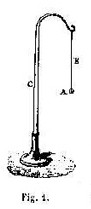
\includegraphics[scale=0.9]{./forces/Mascart01}
\hspace{0.3cm}
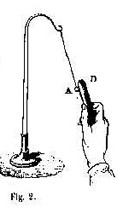
\includegraphics[scale=0.9]{./forces/Mascart02}
\hspace{0.3cm}
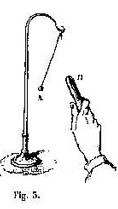
\includegraphics[scale=0.9]{./forces/Mascart03}
\end{center}

L'expérience du pendule électrostatique peut se modéliser par des {\it forces électrostatiques} s'exerçant entre des particules chargées.
%Ce modèle suppose une {\it action à distance}.

%\begin{minipage}[c]{.45\linewidth}
\subsection{Représentation mathématique}
Une charge électrique $Q_1$ exerce une force de Coulomb $\overrightarrow{F}_{Q_1/Q_2}$ sur la charge électrique $Q_2$.
%La force de Coulomb respecte le principe de réaction, la charge électrique $Q_2$ exerce une force de Coulomb $\overrightarrow{F}_{Q_2/Q_1}$ sur la charge électrique $Q_1$.

\begin{center}
\setlength{\unitlength}{1cm}
\begin{picture}(10,3)
\put(0.5,1.0){\circle{0.3}}
\put(0.3,0.3){$Q_1$}
%\put(0.5,1.0){\vector(1,0){1.36}}
%\put(1.2,1.3){$\overrightarrow{F}_{Q_2/Q_1}$}
\put(5.5,1.0){\circle{0.5}}
\put(5.3,0.2){$Q_2$}
\put(5.5,1.0){\vector(-1,0){1.36}}
\put(3.7,1.3){$\overrightarrow{F}_{Q_1/Q_2}$}
\end{picture}
\end{center}
%On peut alors se demander comment l'information de la présence de $Q_1$ parvient à $Q_2$, y a-t-il quelque chose qui se propage entre les charges ? Cette question peut être simplifiée en disant que les charges créent un champ dans tout l'espace et qu'elle sont sensibles à ce champ.
%\end{minipage}\hfill\begin{minipage}[c]{.45\linewidth}

%%%%%%%%%%%%%%%%%%%%%%%%%%%%%%%%%%%%%%%%%%%%%%%%%%%%%%%%%%%%%%%%%%%%%%%%%%%%
